\chapter{反三角函数与简单三角方程的解法}
\section{反正弦函数}
我们知道,正弦函数$y=\sin x$是一个周期等于$2\pi$的振动函
数,它的定义域是$(-\infty,+\infty)$, 而值域是闭区间$[-1,1]$, 它的图象如图9.1。

\begin{figure}[htp]
    \centering
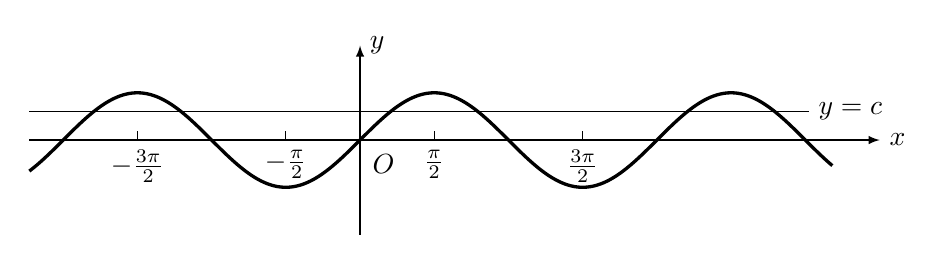
\begin{tikzpicture}[>=latex, scale=.6]
\draw[->] (-7,0)--(11,0)node[right]{$x$};
\draw [->] (0,-2)--(0,2)node[right]{$y$};

\draw[domain=-7:10, samples=1000, very thick] plot(\x,{sin(\x r)});
\draw  (-7,.6)--(9.5,0.6)node[right]{$y=c$};

\foreach \x/\xtext in {-1.5*pi/-\frac{3\pi}{2}, -.5*pi/-\frac{\pi}{2},.5*pi/\frac{\pi}{2}, 1.5*pi/\frac{3\pi}{2}}
{
    \draw (\x,0)node[below]{$\xtext$}--(\x,.2);
}
\node at (.5,-.5){$O$};
\end{tikzpicture}
    \caption{}
\end{figure}


每取一数$y=c,\; -1\le c\le 1$, 作直线$y=c$, 可与正弦曲线
$y=\sin x$交于无穷多个点,这些交点的横坐标是
\[x=x_0+2k\pi\qquad \text{和}\qquad x=(π-x_0)+2k\pi\quad (k\in\mathbb{Z})\]
因此有无数多个$x$的值满足方程$\sin x =c$, 而和那个$y=c$对
应。可见对于变数$x$的一切可能实数值来说,我们不能由函
数$f:\mathbb{R}\to [-1,1]$, $f(x)=\sin x$得出它的反函数来。把定
义域分成无数个单调区间,则在各区间$\left[-\frac{\pi}{2}+2k\pi, \frac{\pi}{2}+2k\pi\right]$上,$y=\sin x$由$-1$上升到1,而在各区间$\left[\frac{\pi}{2}+2k\pi, \frac{3\pi}{2}+2k\pi\right]$上,$y=\sin x$由1下降到$-1$,于是由前一章中的
反函数定理知道,对于上述每一个单调区间存在一个反函数。

如果我们强调的是在闭区间$\left[-\frac{\pi}{2},\frac{\pi}{2}\right]$上
来考虑正弦
函数的反函数,我们就说它是反正弦函数的主值,并把这个函数记作
$x=\arcsin y$,使得
$$x=\arcsin y\qquad \Longleftrightarrow \qquad y=\sin x$$
这里$x\in \left[-\frac{\pi}{2},\frac{\pi}{2}\right],\quad y\in[-1,+1]$。

对于使得$y=\sin x$是单调的另一区间,例如$x\in \left[\frac{\pi}{2},\frac{3\pi}{2}\right]$,
我们就得到另一个反正弦函数。假如我们没有明确地
指出反正弦函数的值域所在的区间,我们就不能由函数$y=\sin x$得出它的反函数。为了明确起见,现在我们规定

\begin{blk}{定义1}
    函数$y=\sin x$在闭区间$\left[-\frac{\pi}{2},\frac{\pi}{2}\right]$上
的反函数
叫做\textbf{反正弦函数}或\textbf{反正弦},这个函数用记号写作
$x=\arcsin y$ (即$x$是一角或弧,其相应的正弦值为$y$),
它的定义域是闭区间$-1\le y\le 1$, 值域是闭区间$-\frac{\pi}{2}\le x\le \frac{\pi}{2}$。
\end{blk}

用习惯上的写法,将字母$x$与$y$互换而写成$y=\arcsin x$,
现在,我们将反正弦函数(主值)的定义用几何名词叙述
如下:

在闭区间$-1\le x\le 1$上,数$x$的反正弦$y=\arcsin x$是在
闭区间$\left[-\frac{\pi}{2},\frac{\pi}{2}\right]$上
的一个角或弧,它的正弦值等于$x$, 
即$\sin y=x$.

由反正弦函数的定义和前一章的反函数定理可得到
它的一些性质如下:
\begin{itemize}
    \item $\arcsin(\sin y)=y,\qquad -\frac{\pi}{2}\le y\le \frac{\pi}{2}$
    
    $\sin(\arcsin x)=x,\qquad -1\le x\le 1$

    \item 函数$f(x)=\arcsin x$在闭区间$[-1,1]$上单调递
    增,并且连续。
    \item $y=\arcsin x,\; -1\le x\le 1$的图象与$y=\sin x,\; -\frac{\pi}{2}\le y\le \frac{\pi}{2}$
    的图象关于直线$y=x$对称(图5.2)。
\end{itemize}

\begin{figure}[htp]
    \centering
\begin{tikzpicture}[>=latex, scale=1]
\draw[->] (-4,0)--(4,0)node[right]{$x$};
\draw [->] (0,-3)--(0,3)node[right]{$y$};

\draw[domain=-pi:pi, samples=1000, dashed, thick] plot(\x,{sin(\x r)});
\draw[domain=-1:1, samples=1000, very thick] plot(\x,{asin(\x)*pi/180});
\draw[dashed] (-3,-3)--(2.5,2.5)node [above]{$y=x$};
\draw [dashed] (0,.5*pi)node[left]{$\frac{\pi}{2}$}--(1,.5*pi)node[above]{$y=\arcsin x$};
\draw [dashed] (0,-.5*pi)node[right]{$-\frac{\pi}{2}$}--(-1,-.5*pi);
\node at (.25,-.25){$O$};
\node at (pi+.5,0)[above]{$y=\sin x$};
\foreach \x in {-1,1}
{
    \draw (\x,0)node[below]{$\x$}--(\x,.1);
}
\draw (0,1)node[left]{$1$}--(.1,1);
\draw (0,-1)--(-.1,-1)node[right]{$-1$};

\end{tikzpicture}
    \caption{}
\end{figure}



我们已知正弦函数是奇函数,它的图象关于原点对称,
现在我们要证明 $f(x)=\arcsin x$是奇函数,即
$\arcsin(-x)=-\arcsin x$。

\begin{proof}
    因为$-\frac{\pi}{2}\le \arcsin x\le \frac{\pi}{2}$,
    角$-\arcsin x$也被限制在由$-\frac{\pi}{2}$到$\frac{\pi}{2}$
    的区间内:
    $$-\frac{\pi}{2}\le -\arcsin x\le \frac{\pi}{2}$$
    又,角$-\arcsin x$的正弦等于$-x$
\[\sin(-\arcsin x)=-\sin(\arcsin x)=-x\]
因此:$\arcsin(-x)=-\arcsin x$。
\end{proof}

\begin{example}
    求下列各式的值(口答):
    \begin{enumerate}
        \item $\arcsin\frac{1}{2}$
        \item $\arcsin\left(-\frac{1}{2}\right)$
        \item $\arcsin 1$
    \end{enumerate}
\end{example}

\begin{solution}
\begin{enumerate}
    \item $\arcsin\frac{1}{2}=\frac{\pi}{6}$,因为$\sin\frac{\pi}{6}=\frac{1}{2}$,且$-\frac{\pi}{2}<\frac{\pi}{6}<\frac{\pi}{2}$

    \item $\arcsin\left(-\frac{1}{2}\right)=-\frac{\pi}{6}$,因为$\sin\left(-\frac{\pi}{6}\right)=-\frac{1}{2}$,且
    $-\frac{\pi}{2}<-\frac{\pi}{6}<\frac{\pi}{2}$
    \item $\arcsin 1=\frac{\pi}{2}$,因为$\sin\frac{\pi}{2}=1$,而且$\frac{\pi}{2}$不超出$\left[-\frac{\pi}{2},\frac{\pi}{2}\right]$的界限。
\end{enumerate}
\end{solution}

\begin{example}
    求下列各式的值:
\[\arcsin\left(-\frac{\sqrt{3}}{2}\right),\qquad \arcsin (-0.2672) \]
\end{example}

\begin{solution}
\begin{enumerate}
    \item $\arcsin\left(-\frac{\sqrt{3}}{2}\right)=-\arcsin\frac{\sqrt{3}}{2}=-\frac{\pi}{3}$
    \item $\arcsin(-0.2672)=-\arcsin0.2672=-15^{\circ}30'\approx -0.2705$
\end{enumerate}
    
\end{solution}



\begin{example}
    求下列各式的值:
\begin{multicols}{2}
\begin{enumerate}
    \item $\sin\left(\arcsin\frac{1}{3}\right)$
    \item $\tan\left(\arcsin\frac{\sqrt{2}}{2}\right)$
    \item $\cos\left(\arcsin\frac{3}{5}\right)$
    \item $\sin\left[2\arcsin\left(-\frac{3}{5}\right)\right]$
    \item $\arcsin\left(\sin\frac{7\pi}{6}\right)$
\end{enumerate}
\end{multicols}
\end{example}

\begin{solution}
\begin{enumerate}
    \item $\sin\left(\arcsin\frac{1}{3}\right)=\frac{1}{3}$
    \item $\tan\left(\arcsin\frac{\sqrt{2}}{2}\right)=\tan\frac{\pi}{4}=1$
    \item 设$\arcsin\frac{3}{5}=\alpha$,其中$-\frac{\pi}{2}\le\alpha\le\frac{\pi}{2}$,那么$\sin\alpha=\frac{3}{5}$。由于$-\frac{\pi}{2}\le\alpha\le\frac{\pi}{2}$,$\sin\alpha>0$,可以知道,$\alpha$是第一象限的角,所以
    $$\cos\left(\arcsin\frac{3}{5}\right)=\sqrt{1-\left(\frac{3}{5}\right)^2}=\frac{4}{5}$$
    \item 设$\arcsin\left(-\frac{3}{5}\right)=\alpha$,其中$-\frac{\pi}{2}\le\alpha\le\frac{\pi}{2}$,那么
    \[\sin\alpha =\sin\left[\arcsin\left(-\frac{3}{5}\right)\right]=-\frac{3}{5}\]
由于$-\frac{\pi}{2}\le\alpha\le\frac{\pi}{2}$和$\sin\alpha<0$,可以知道$\alpha$是第四象限的角,所以
\[\cos\alpha=\sqrt{1-\left(-\frac{3}{5}\right)^2}=\frac{4}{5}\]
即:
$\sin\left[2\arcsin\left(-\frac{3}{5}\right)\right]=\sin2\alpha=2\sin\alpha\cdot \cos\alpha=2\left(-\frac{3}{5}\right)\cdot\left(\frac{4}{5}\right)=-\frac{24}{25}$
    \item \[\begin{split}
\arcsin\left(\sin\frac{7\pi}{6}\right)&=\arcsin\left[\sin\left(\pi+\frac{\pi}{6}\right)\right]\\
&=\arcsin\left(-\sin\frac{\pi}{6}\right)\\
&=-\arcsin\left(\sin\frac{\pi}{6}\right)=-\frac{\pi}{6}        
    \end{split}\]
\end{enumerate}
\end{solution}

关于$y=\sin x$, 只要知道了它在闭区间$-\frac{\pi}{2}\le x\le \frac{\pi}{2}$上
的反函数$x=\arcsin y$, 我们便能求出$y=\sin x$在其它单调区间
上的反函数。

\begin{blk}{命题}
\begin{enumerate}
    \item $y=\sin x$在闭区间$\left[-\frac{\pi}{2}+2k\pi,\frac{\pi}{2}+2k\pi\right]$上,由$-1$上升到1,它们相应的反函数是
\[x=\arcsin y+2k\pi,\quad k\in\mathbb{Z}\]
因为
\[\sin x= \sin(\arcsin y+ 2k\pi) = \sin(\arcsin y) = y\]
而且
\[-\frac{\pi}{2}+2k\pi\le \arcsin y+2k\pi \le \frac{\pi}{2}+2k\pi
,\quad k\in\mathbb{Z}\]
    
\item $y=\sin x$在闭区间$\left[\frac{\pi}{2},\frac{3\pi}{2}\right]$上,由1下降到$-1$,
它的反函数是
\[x=\pi-\arcsin y\]
因为
\[\sin x=\sin(\pi- \arcsin y) = \sin(\arcsin y) = y\]
而且
\[\frac{\pi}{2}=\pi-\frac{\pi}{2} \le \pi-\arcsin y \le \pi+\frac{\pi}{2}=\frac{3\pi}{2}\]
我们也可以在单位圆上作图来说明2,如图9.3所示。

\item $y=\sin x$在闭区间$\left[\frac{\pi}{2}+2k\pi,\frac{3\pi}{2}+2k\pi\right]$上,由
1下降到$-1$, 相仿地证得它在相应区间上的反函数是
\[x=(\pi-\arcsin y)+2k\pi,\quad k\in\mathbb{Z} \]
\end{enumerate}
\end{blk}

\begin{figure}[htp]
    \centering
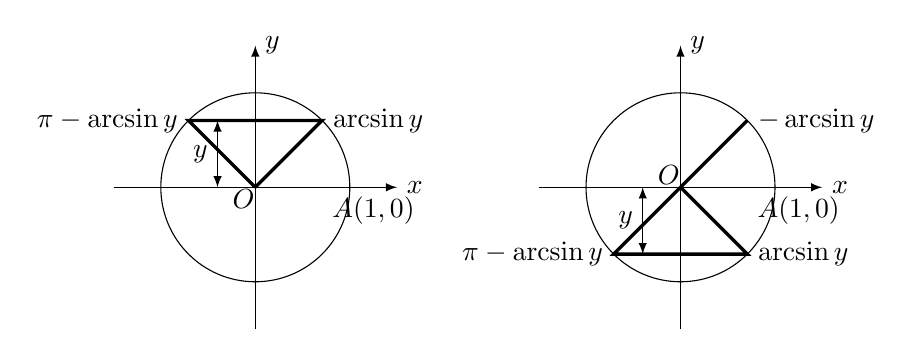
\begin{tikzpicture}[>=latex, scale=.6]
\begin{scope}
    \draw[->] (-3,0)--(3,0)node[right]{$x$};
    \draw[->] (0,-3)--(0,3)node[right]{$y$};
    \draw (0,0) circle(2);
    \node at (-.25,-.25){$O$};
\node at (2.5,0)[below]{$A(1,0)$};
\draw[very thick] (0,0)--(45:2)node[right]{$\arcsin y$}--(90+45:2)node[left]{$\pi-\arcsin y$}--(0,0);

\draw[<->] (-.8,0)--node[left]{$y$}(-.8,1.414);
\end{scope}

\begin{scope}[xshift=9cm]
    \draw[->] (-3,0)--(3,0)node[right]{$x$};
    \draw[->] (0,-3)--(0,3)node[right]{$y$};
    \draw (0,0) circle(2);
    \node at (-.25,.25){$O$};
\node at (2.5,0)[below]{$A(1,0)$};

\draw[<->] (-.8,0)--node[left]{$y$}(-.8,-1.414);
\draw[very thick] (0,0)--(-45:2)node[right]{$\arcsin y$}--(-90-45:2)node[left]{$\pi-\arcsin y$}--(0,0);
\draw[very thick] (0,0)--(45:2)node[right]{$-\arcsin y$};
\end{scope}
\end{tikzpicture}

    \caption{}
\end{figure}


\begin{example}
    讨论函数$y=\arcsin(\sin x)$的图象。
\end{example}

\begin{solution}
    由于正弦的周期性,函数$\arcsin(\sin x),\; x\in\mathbb{R}$也以
$2\pi$为周期,因此,只研究它在长度为$2\pi$的区间内情形即可。
由于
\[\sin y=\sin[\arcsin(\sin x)]=\sin x\]
这里$-\frac{\pi}{2}\le y\le \frac{\pi}{2}$,而$x\in\mathbb{R}$,故
\begin{itemize}
    \item 当$x\in\left[-\frac{\pi}{2},\frac{\pi}{2}\right]$时,则$y=x$。
    \item 当$x\in\left[\frac{\pi}{2},\frac{3\pi}{2}\right]$时,则由上面的命题2知
    \[x=\pi-y\quad \Rightarrow\quad y=\pi-x\in \left(-\frac{\pi}{2},\frac{\pi}{2}\right)\]
\end{itemize}
因之,在此区间内函数的图象与直线$y=\pi-x$一致,总之,
由上面的命题中的1和3的结果:
\begin{enumerate}
    \item 当$x\in \left[-\frac{\pi}{2}+2k\pi,\frac{\pi}{2}+2k\pi\right]$时,则$x=y+2k\pi$,则$y=x-2k\pi$;
    \item 当$x\in \left[\frac{\pi}{2}+2k\pi,\frac{3\pi}{2}+2k\pi\right]$时,则$x=\pi-y+2k\pi$,则$y=(\pi-x)-2k\pi$。
\end{enumerate}
由上面讨论的结果,得到函数$y= \arcsin
(\sin x)$的图象是折线的形状,如图5.4所示。
\begin{figure}[htp]
    \centering
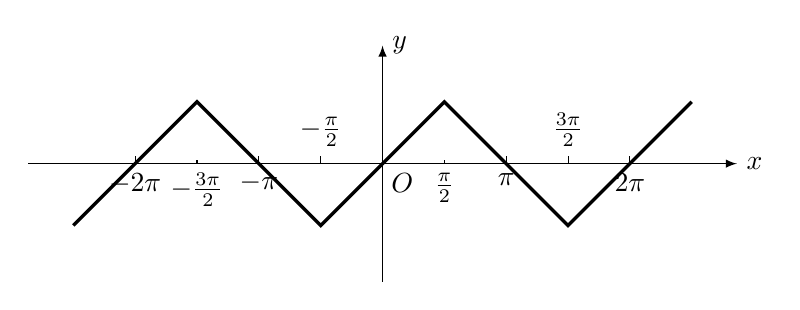
\begin{tikzpicture}[>=latex, scale=.5]
    \draw[->] (-9,0)--(9,0)node[right]{$x$};
    \draw[->] (0,-3)--(0,3)node[right]{$y$};
\draw[very thick] (-2.5*pi,-0.5*pi)--(-1.5*pi,.5*pi)--(-.5*pi,-0.5*pi)--(.5*pi,.5*pi)--(1.5*pi,-0.5*pi)--(2.5*pi,.5*pi);
\foreach \x/\xtext in {-2/-2\pi, -1/-\pi,1/\pi,2/2\pi}
{
    \draw (pi*\x,0)node[below]{$\xtext$}--(pi*\x,0.2);
}
\foreach \x/\xtext in {.5/\frac{\pi}{2},-1.5/-\frac{3\pi}{2}}
{
    \draw (pi*\x,0)node[below]{$\xtext$}--(pi*\x,0.1);
}
\foreach \x/\xtext in {1.5/\frac{3\pi}{2},-.5/-\frac{\pi}{2}}
{
    \draw (pi*\x,0)--(pi*\x,0.2)node[above]{$\xtext$};
}
\node at (.5,-.5){$O$};

\end{tikzpicture}
    \caption{}
\end{figure}
\end{solution}



\section*{习题9.1}
\addcontentsline{toc}{subsection}{习题9.1}
\begin{enumerate}
    \item 用反三角函数表示下面等式中的角。
    \begin{multicols}{2}
\begin{enumerate}
    \item $\sin\frac{\pi}{4}=\frac{\sqrt{2}}{2}$
    \item $\sin\frac{5\pi}{3}=-\frac{\sqrt{3}}{3}$
    \item $\sin\frac{7\pi}{3}=\frac{\sqrt{3}}{2}$
    \item $\sin(-2.314)=-0.04038$
\end{enumerate}
    \end{multicols}
    \item 当$\frac{1}{2}\le x\le\frac{\sqrt{3}}{2}$
    时,求函数$y=x\arcsin x$的最大值
    和最小值。
    \item 不求值,确定下面差的符号:
\begin{enumerate}
    \item $\arcsin 0.7-\arcsin 0.5$
    \item $\arcsin\left(-\frac{3}{5}\right)-\arcsin\left(-\frac{3}{4}\right)$
    \item $\arcsin\left(\sqrt{2}-1\right)-\arcsin\left(\sqrt{5}-2\right)$
\end{enumerate}
\item 求下列各式的值:
\begin{multicols}{2}
\begin{enumerate}
    \item $\arcsin\frac{\sqrt{3}}{2}$
    \item $\arcsin\left(-\frac{\sqrt{2}}{2}\right)$
    \item $\arcsin0$
    \item $\arcsin(-1)$
    \item $\arcsin\left(-\frac{1}{4}\right)$
    \item $\arcsin0.7841$
\end{enumerate}
\end{multicols}

\item 计算下列各式的值:
\begin{multicols}{2}
    \begin{enumerate}
        \item $\tan\left(\arcsin\frac{\sqrt{2}}{2}\right)$
        \item $\cos\left(\arcsin \frac{3}{5}\right)$
        \item $\arcsin \left[\sin\left(-\frac{\pi}{7}\right)\right]$
        \item $\arcsin\left(\sin\frac{5\pi}{6}\right)$
        \item $\arcsin(\cos1)$
    \end{enumerate}
    \end{multicols}
    \item 计算下列各式的值:
\begin{multicols}{2}
    \begin{enumerate}
        \item $\cot\left(2\arcsin\frac{\sqrt{2}}{2}\right)$
        \item $\cos\left(2\arcsin\frac{1}{3}\right)$
        \item $\sin\left(3\arcsin\left(-\frac{\sqrt{3}}{2}\right)\right)$
        \item $\tan\left(\frac{1}{2}\arcsin\frac{2}{3}\right)$
    \end{enumerate}
    \end{multicols}

    \item 讨论函数$y=x \arcsin(\sin x)$的图象,并作草图。
\item 画出$f(x)=\sin(3\arcsin x)$的图象。
\end{enumerate}























































































































































































